\documentclass{report}

\usepackage[ngerman]{babel}
\usepackage[utf8]{inputenc}
\usepackage[T1]{fontenc}
\usepackage{hyperref}
\usepackage{csquotes}
\usepackage[a4paper]{geometry}
\usepackage{graphicx}
\usepackage{float}
\usepackage{caption}
\usepackage{url}

\usepackage[
    backend=biber,
    style=apa,
    sortlocale=de_DE,
    natbib=true,
    url=true,
    doi=false,
    sortcites=true,
    sorting=nyt,
    isbn=false,
    hyperref=true,
    backref=false,
    giveninits=false,
    eprint=false]{biblatex}
\addbibresource{../references/bibliography.bib}


\title{Ist der Einsatz von KI im Gesundheitswesen ethisch vertretbar?}
\author{Käthe Linke Aguirre}
\date{31.5.2024}


\begin{document}

\maketitle

\abstract{
In diesem Dokument werde ich die Frage untersuchen, ob der Einsatz von 
Künstlicher Intelligenz (KI) ethisch vertretbar ist und welche
Möglichkeiten und Herausforderungen damit verbunden sind.
}

\tableofcontents

\chapter{Einleitung}

\section{Was ist KI?}
  
Künstliche Intelligenz (KI) ist die Fähigkeit einer Maschine, menschliche Fähigkeiten
wie logisches Denken, Lernen, Planen und Kreativität zu imitieren. KI ist einer der 
grossen technologischen Fortschritte unserer Zeit. Ihre Entwicklung schreitet 
rasant voran und die Einsatzmöglichkeiten nehmen zu. KI ist ein wichtiger Bestandteil nicht nur in der 
Informatik,sondern auch vieler anderer Bereiche unseres Lebens. 
\newline
KI wird zum Beispiel,... 
\begin{enumerate}
    \item in der Bildung verwendet. Adaptive Lernplatformen wie Knewton, Quizlet und Duolingo
    bieten Nutzer individuelle Lernsysteme. Sie können mit automatisierten Tutoren den Schülern bei 
    ihren Aufgaben helfen.
    \item in der Architektur verwendet. Sie kann zum Beispiel Gebäudeentwürfe generieren.
    \item in der Kunst verwendet. KI kann mithilfe von generativen Modellen Kunstwerke erstellen.
    Mit KI-Programmen kann man zum Beispiel Musik komponieren.
    \item in der Medizin verwendet. KI kann verwendet werden um Krankheiten zu diagnostizieren. 
    Es kann auch genutzt werden um relevante Muster in digitalisierten medizinischen 
    Daten zu finden und präzise Entscheidungen zu treffen.
\end{enumerate}

\begin{figure*}
    \centering
    
\includegraphics[width=0.55\textwidth]{R.jpg}
    \label{fig:R}
    \caption{Kontakt zwischen Mensch und KI}
    \end{figure*}

    \addcontentsline{lof}{figure}{\protect\numberline{\ref{fig:R}}Kontakt zwischen Mensch und KI (Quelle:\protect\url{https://www.bing.com/images/search?view=detailV2&insightstoken=bcid_RC4R44y8XBkHHJSsqAgBWJrG3.wJ.....0Q*ccid_LhHjjLxc&form=SBIIRP&iss=SBIUPLOADGET&sbisrc=ImgDropper&idpbck=1&sbifsz=976+x+500+·+44.21+kB+·+jpeg&sbifnm=R.jpg&thw=976&thh=500&ptime=64&dlen=60360&expw=838&exph=429&selectedindex=0&id=487381842&ccid=LhHjjLxc&vt=2&sim=11}))}


    \newpage
\section {Wie wird KI trainiert?}

KI-Modelle werden in der Regel durch einen Prozess des maschinellen Lernens trainiert, 
der in drei Hauptschritte unterteilt werden kann. Der Trainingprozess beginnt mit der Datensammlung, 
bei der ein Computeralgorithmus mit einer grossen Menge an Daten gefüttert wird, die für die Erstellung 
von Vorhersagen und deren Genauigkeit notwendig sind. Diese Daten können strukturiert (z.B. Tabellen) oder 
unstrukturiert (z.B. Texte) sein. Während des Trainings wird dem Modell beigebracht, verschiedene Merkmale 
in den Daten zu erkennen, indem es seine internen Parameter anpasst, um Fehler bei der Vorhersage 
zu minimieren. \\ Im zweiten Schritt findet ein Validierungsprozess statt, bei dem bewertet wird, wie gut 
das trainierte Modell seine Fähigkeiten auf ihm unbekannte Daten anwenden kann. Schliesslich wird das Modell mit neuen, bisher 
ungesehenen Daten getestet, um zu überprüfen, ob es genaue Vorhersagen treffen kann oder nicht. 
\citep{clickworker}
\\
Jedoch ist zu beachten, dass bei der Datensammlung und Datenverwendung Datenschutzrichtlinien und -gesetze 
eingehalten werden müssen um sicherzustellen, dass die Privatsphäre und die Rechte von Personen respektiert 
werden. Ein anderer wichtiger Aspekt, der beachtet werden muss, ist dass die Funktionsweise und die 
Entscheidungen, die das System trifft, verständlich und nachvollziehbar sind. Ist das nicht der Fall, 
dann können Probleme wie Skepsis und Ablehnung auftreten. 


\chapter{KI im Gesundheitswesen}


\section{Wofür wird KI im Gesundheitswesen verwendet?}

Künstliche Intelligenz (KI) hat bereits viele Bereiche im Gesundheitswesen beeinflusst. Sie bietet nicht nur 
vielfältige Möglichkeiten sondern auch Herausforderungen.\\ Einige Gebiete wo KI eine bedeutende Rolle spielt sind:


\begin{enumerate}
    \item \underline{Diagnostik:} \\KI-Systeme unterstützen Ärzte bei der schnelleren und präziseren Diagnose 
    von Krankheiten, indem sie Muster in medizinischen Bildern, Labortests und Patientendaten erkennen.
    Bspw. können sie Anomalien auf Röntgenbildern oder MRT-Scans identifizieren, die für das menschliche 
    Auge schwer erkennbar sind.
    \item \underline{Prognostik:} \\KI-Software kann auch zur Entwicklung neuer Therapien und Medikamente beitragen. 
    Durch die Analyse grosser Datenmengen aus klinischen Studien und Patientendaten können KI-Algorithmen 
    Trends und Muster erkennen, die auf wirksamere Behandlungsmethoden hinweisen. Dadurch können Forscher 
    personalisierte Behandlungsansätze entwickeln, die besser auf die individuellen Bedürfnisse der 
    Patienten abgestimmt sind. 
    \item \underline{Behandlungsplanung und -unterstützung:} \\KI-gesteuerte Roboter werden immer häufiger in
    Operationssälen eingesetzt, um die Präzision und Sicherheit zu verbessern. Diese Roboter können
    die Bewegungen des Chirurgen verfeinern und gleichzeitig das Risiko menschlicher Fehler minimieren. 
    Dadurch können komplexere Operationen durchgeführt und die Erholungszeit der Patienten verkürzt werden. \citep{mauriceneumann.de}
\end{enumerate} 

\begin{figure}[H]
    \centering
    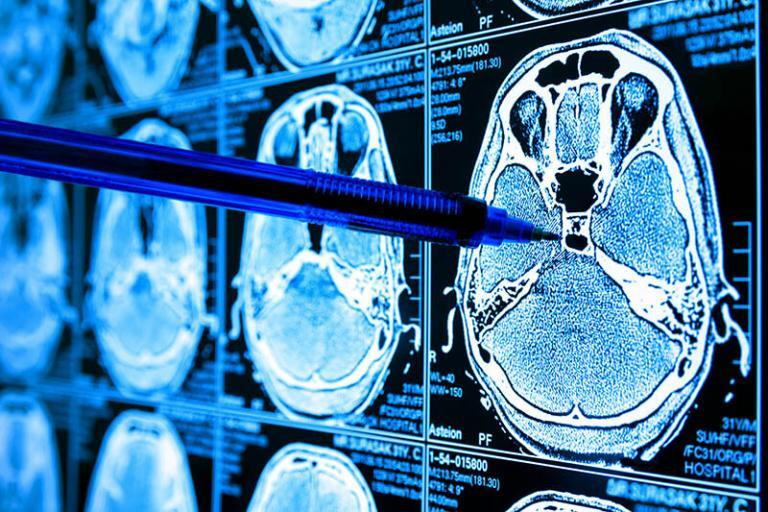
\includegraphics[width=0.32\textwidth]{fotitooppa.jpg}
    \label{fig:fotitooppa}
    \caption{Dieses Bild zeigt auf, wie KI im Gesundheitswesen verwendet wird.}
\end{figure}

\addcontentsline{lof}{figure}{\protect\numberline{\ref{fig:fotitooppa}}Dieses Bild zeigt auf, wie KI im Gesundheitswesen verwendet wird. (Quelle: \protect\url{https://sciencemediahub.eu/2021/11/17/the-future-of-ai-in-medical-imaging/})}

Bei der Anwendung von KI im Gesundheitsbereich, werden Medizin-\\produkte und Nicht-Medizinprodukte 
unterschieden. Dies basiert auf ihrem Verwendungszweck, ihrer Regulierung und ihren Funktionen.

\begin{itemize}
\item \underline{Nicht-Medizinprodukte:}\\ Dies umfasst Geräte, Software oder Anwendungen, die 
der Gesundheit und dem Wohlbefinden des Menschen dienen, jedoch keine medizinische Zweckbestimmung haben oder nicht an Menschen 
eingesetzt werden. Sie müssen weniger strengen Vorschriften, jedoch grundlegenden Sicherheits- und Datenschutzstandards
einhalten. Beispiele: Fitness-Apps und Wearables.
\item \underline{Medizinprodukte:} \\Dies sind Geräte, Software oder Anwendungen die speziell für medizinische Zwecke 
entwickelt und verwendet werden. Sie werden zur Diagnose, Behandlung oder Überwachung von Krankheiten eingesetzt.
Um sicher und effektiv zu sein, müssen sie strenge Vorschriften einhalten und häufig behördliche Genehmigungen wie die der EMA 
in Europa erhalten. Beispiele: diagnostische Geräte wie MRTs und Blutzuckermessgeräte sowie therapeutische Geräte
wie Beatmungsgeräte.
\end{itemize}

\begin{figure}[H]
    \centering
    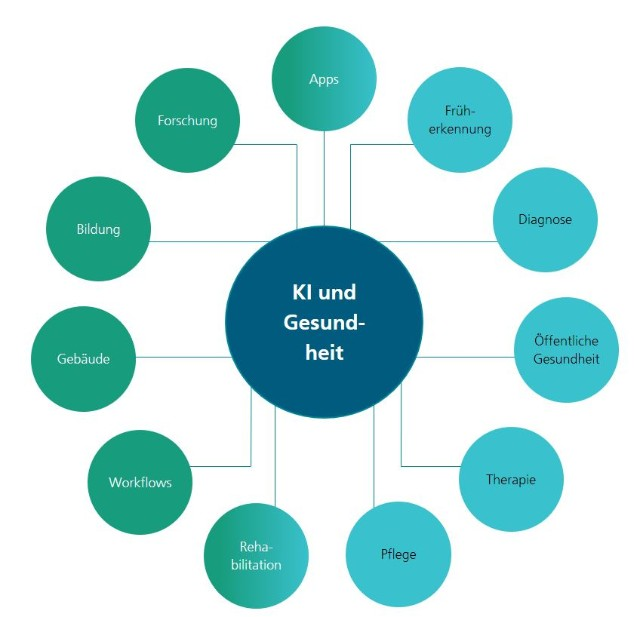
\includegraphics[width=0.50\textwidth]{Bild13.jpg}
    \caption{Dieses Bild soll das Spektrum der Anwendungen von KI im Gesundheitsbereich darstellen. Die rechte Seite des Spektrums (türkis eingefärbt)
    zeigt die Medizinprodukten auf. Auf der linke Seite (grün eingefärbt) werden die Nicht-Medizinprodukten aufgezeigt.}

    \label{fig:Bildmedizin}
\end{figure}

    \addcontentsline{lof}{figure}{\protect\numberline{\ref{fig:Bildmedizin}}Dieses Bild soll das Spektrum der Anwendungen von KI im Gesundheitsbereich darstellen. (Quelle: \protect\url{https://www.isi.fraunhofer.de/de/blog/2023/kuenstliche-intelligenz-im-gesundheitsbereich.html})}


\newpage
\subsection {Ist KI in der Medizin ethisch vertretbar oder nicht?}

Ethik spielt in vielen Bereichen unseres Lebens eine zentrale Rolle, insbesondere 
im Gesundheitswesen, wo Entscheidungen über Leben und Tod getroffen werden. 
Wie ich vorhin gezeigt habe, bietet KI in vielen Bereichen im Gesundheitswesen viele Möglichkeiten, wie beispielsweise
die Fähigkeit, Forschern umfangreiche Daten aus verschiedenen Quellen zu sammeln und eine
genau Analyse lebensbedrohlicher Krankheiten zu ermöglichen. Sie kann auch durch automatisierte Aufgaben einen schnellen 
Datenaustausch und organisierte Abläufe dazu beitragen, den Stress des medizinische Fachpersonals zu verringern.
Doch mit diesen Fortschritten kommen auch wichtige ethische, rechtliche und soziale 
Fragen auf, die sich um den Datenschutz und die Verantwortung bei Entscheidungen zwischen Mensch und Maschine drehen.
\\
Künstliche Intelligenz (KI) ermöglicht es, eine Analyse von Krankheitsdaten
genauere Diagnosen und Prognosen zu erstellen. Jedoch müssen zuerst Gesundheitsdaten von Patienten gesammelt und
gespeichert werden, um diese Erkenntnisse zu gewinnen. Obwohl dies ein grosser Vorteil ist, können jedoch Probleme
hinsichtlich des Datenschutzes und der Sicherheit auftreten, da sich mit die fortschreitender Technologie auch 
Cyberangriffe immer weiter entwickeln.\citep{clutch} Um solche Sorgen und Probleme zu verhindern, muss sichergestellt werden,
dass die persönliche Gesundheitsdaten von Patienten angemessen geschützt und anonymisiert werden, um ihre Privatsphäre 
zu bewahren.
\\
Neben den Problemen des Datenschutzes und der Sicherheit können auch Herausforderungen bei der Entscheidungsfindung in der Behandlungsplanung auftreten, wenn KI-gestützte
Patientendiagnose verwendet werden. KI sind darauf angewiesen, aus den gesammelten und gespeicherten Daten, 
Krankheiten bei Patienten zu identifizieren. Tritt aber der Fall auf, dass unzureichende Daten zu bestimmten Krankheiten 
vorliegen, kann dies zu eine Fehldiagnose führen. Dies gefährdet nicht nur das Leben des Patienten, sondern stellt das medizinische 
Fachpersonal vor erhebliche Schwierigkeiten. Solche Fehldiagnosen können seitens der Bevölkerung zu Skepsis und Ablehnung in die Technologie führen
und somit die Verantwortung für medizinische Entscheidungen verkomplizieren. Deswegen ist es von entscheidender Bedeutung, 
dass KI-Systeme kontinuierlich mit aktuellen und umfassenden Daten gefüttert werden, kontinuierlich überwacht und angepasst werden, um sicherzustellen, dass sie korrekt und zuverlässig funktionieren
und die endgültige Diagnose von einem wirklichen Arzt überprüft wird. Nur so kann man gewährleisten, dass die Vorteile
der KI im Gesundheitswesen sicher und effektiv genutzt werden. 

\subsection {Fazit}

Insgesamt zeigt sich, dass der Einsatz von Künstlicher Intelligenz im Gesundheitswesen sowohl Chancen
und Herausforderungen mit sich bringen kann. Während KI die Effizienz, Genauigkeit und Verfügbarkeit
von Gesundheitsdienstleistungen verbessern kann, muss man gleichzeitig ethische, rechtliche und soziale Fragen angemessen berücksichtigen.
Datenschutz, Sicherheit und die menschliche Verantwortung bei Entscheidungen sind von entscheidender Bedeutung. Man muss sicherstellen,
dass die Daten von Patienten angemessen gesichert und privat bleiben und dass KI-gestützte
Diagnosen und Entscheidungen immer von menschlichen Fachkräften überprüft und geleitet werden. Nur auf diese Weise
kann man sicherstellen, dass die Anwendung von KI ethisch vertretbar bleibt.



\printbibliography
\listoffigures


\end{document}

